\subsection{Anwendung}\label{sec:ladeablauf}
Nachdem die Unterteilung zwischen Betreiber und User gemacht wurde, kann nun die Betriebsebene verdeutlicht werden. Um einen lückenlosen Betrieb zu gewährleisten, ist ein Konzept für den Ablauf von Vorteil. Nachfolgend werden die Hauptschritte erklärt. Abbildung \ref{fig:Anwendungsablauf Dojo} dient zur Übersicht und zeigt einen möglichen Anwendungsablauf.

\begin{figure}[H]
	\begin{center}
		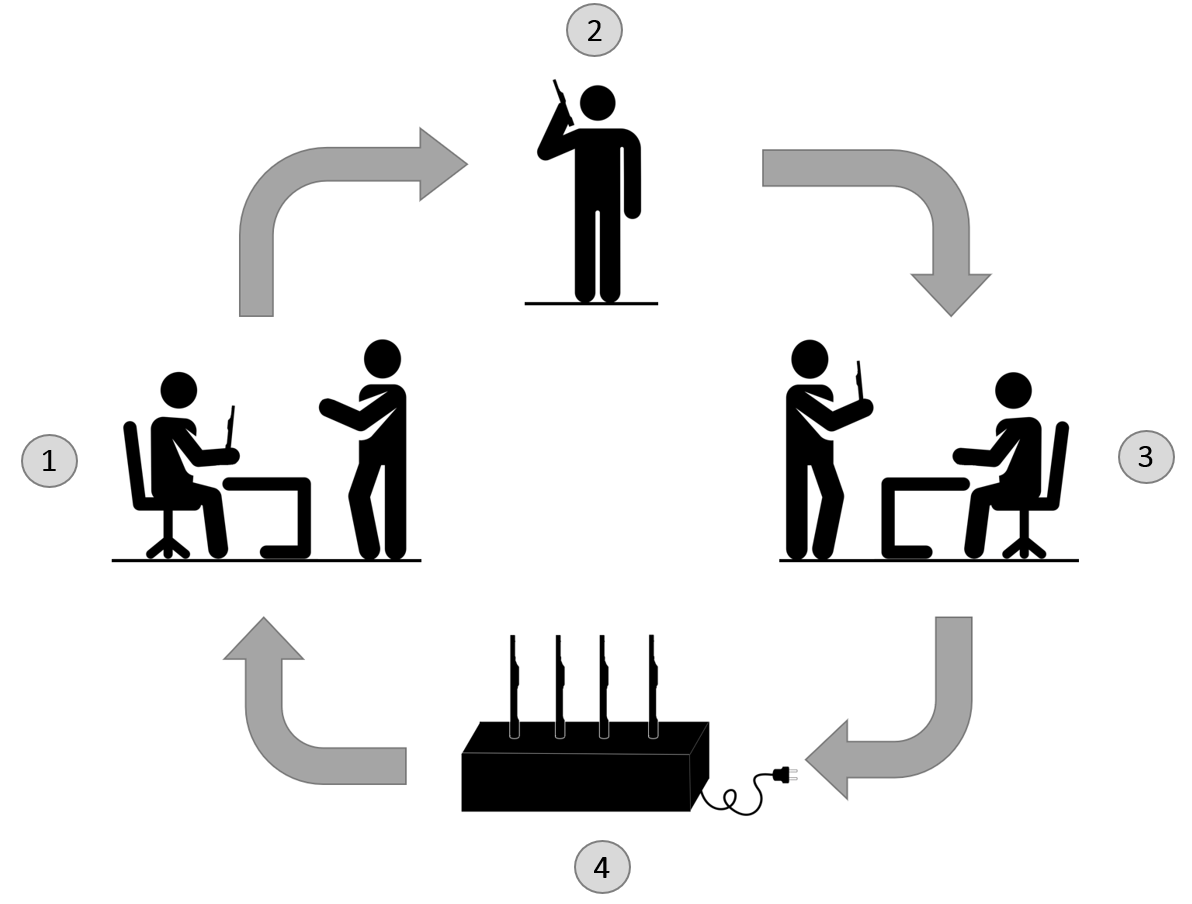
\includegraphics[width=120mm]{data/Ladezyklus.png}
		\caption[Anwendungsablauf des Dōjōs]{Anwendungsablauf im Museum} %picture caption
		\label{fig:Anwendungsablauf Dojo}
	\end{center}
\end{figure}

\textbf{Schritt 1} beinhaltet die Ausgabe des Dōjōs am Empfang. Es werden jeweils die Geräte mit dem höchsten Ladestatus abgegeben. Ein lückenloser Betrieb wird erreicht, wenn die Stückzahl der Audio-Guides in etwa der Anzahl Besucher pro Tag entspricht. Die Zutrittsberechtigung wird gemäss dem Wunsch des Besuchers festgelegt. Anschliessend wird die Sprache durch den Besucher selbst gewählt. Hierbei stehen ihm vier Bluetooth-Beacons zur Verfügung, zu welchen er sein Dōjō hinhalten kann. Die gewünschte Sprache ist hierbei durch die Landesflagge gekennzeichnet. Abbildung \ref{fig:SprachauswahlBeacon} zeigt das Prinzip. Damit eine der vier Sprachen auf dem Dōjō aktiviert wird, muss das Gerät an den richtigen Beacon gehalten werden und gleichzeitig die Play-Taste gedrückt werden. Wurde die Sprache erfolgreich ausgewählt, wird ein kurzes Audio-Sample zur Überprüfung der gewählten Sprache abgespielt. Sobald die gewünschte Sprache geladen und getestet wurde, kann der Museumsbesuch gestartet werden.

In \textbf{Schritt 2} befindet sich der Besucher auf dem Rundgang mit dem Dōjō. Dabei hat er die Möglichkeit, während dem Rundgang Bilder zu \glqq liken\grqq und sich die zugehörigen Audio-Files der Kunstobjekte anzuhören.

Die Abgabe der Gerätes erfolgt in \textbf{Schritt 3}. Hier hat der Besucher die Möglichkeit die Kunstobjekte, welche mit einem {\glqq Like\grqq} versehen wurden, als Broschüre oder per Mail zu erhalten. Der entgegengenommene Dōjō kann nun für den nächsten Besucher gereinigt werden.

In \textbf{Schritt 4} werden alle benötigten Informationen extrahiert. Danach wird das Gerät mit der induktiven Ladestation geladen. Für weitere Informationen zur Ladestation wird auf das Kapitel \ref{sec:energieuebertragung} verwiesen. Nun kann der Zyklus wieder von vorne beginnen.
\begin{figure}[H]
	\begin{center}
		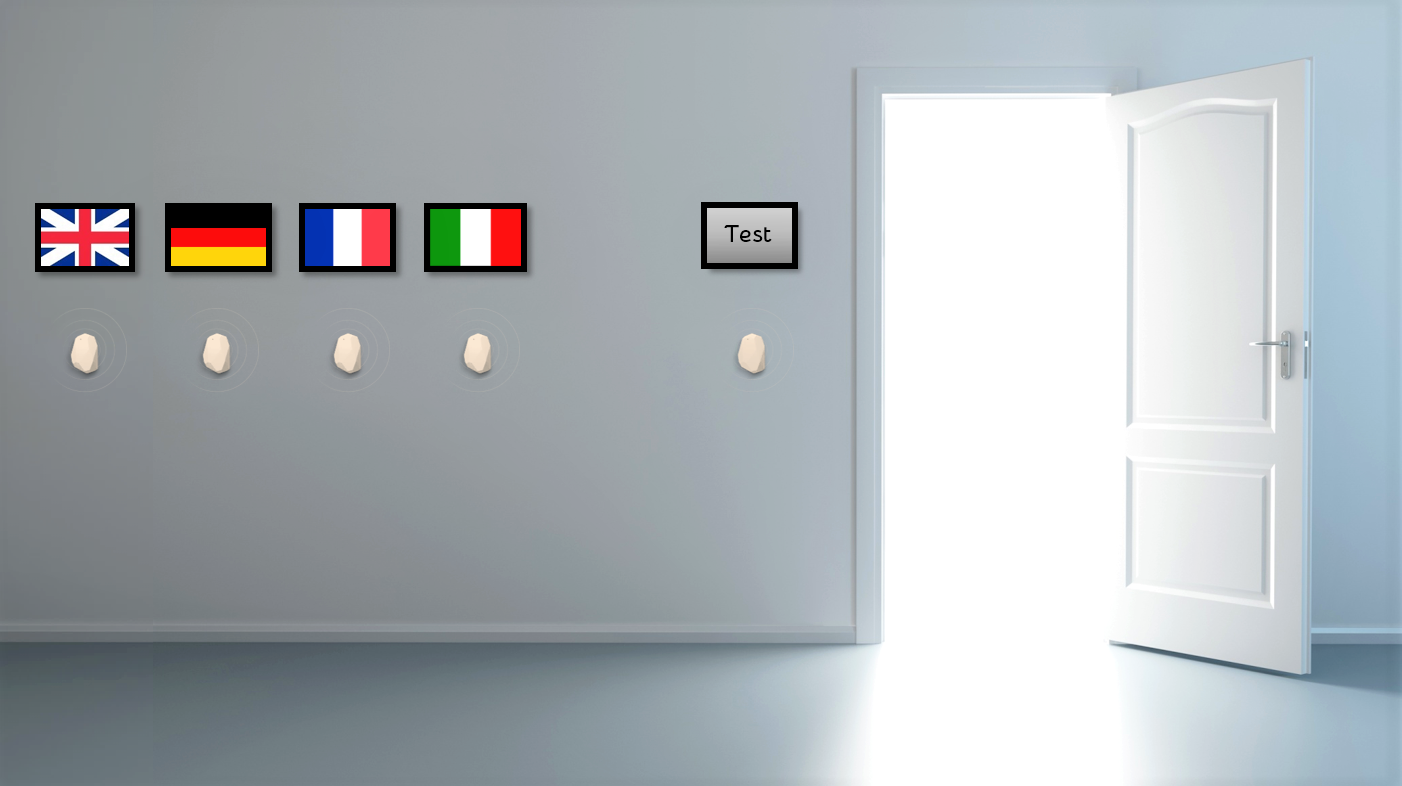
\includegraphics[width=140mm]{data/BeaconSpracherkennung.png}
		\caption[Sprachauswahl mittels Bluetooth-Beacon]{Sprachauswahl mittels Bluetooth-Beacon} %picture caption
		\label{fig:SprachauswahlBeacon}
	\end{center}
\end{figure}